\begin{tikzpicture}
	\onslide<4->{ \node[] (input_taj) 
		{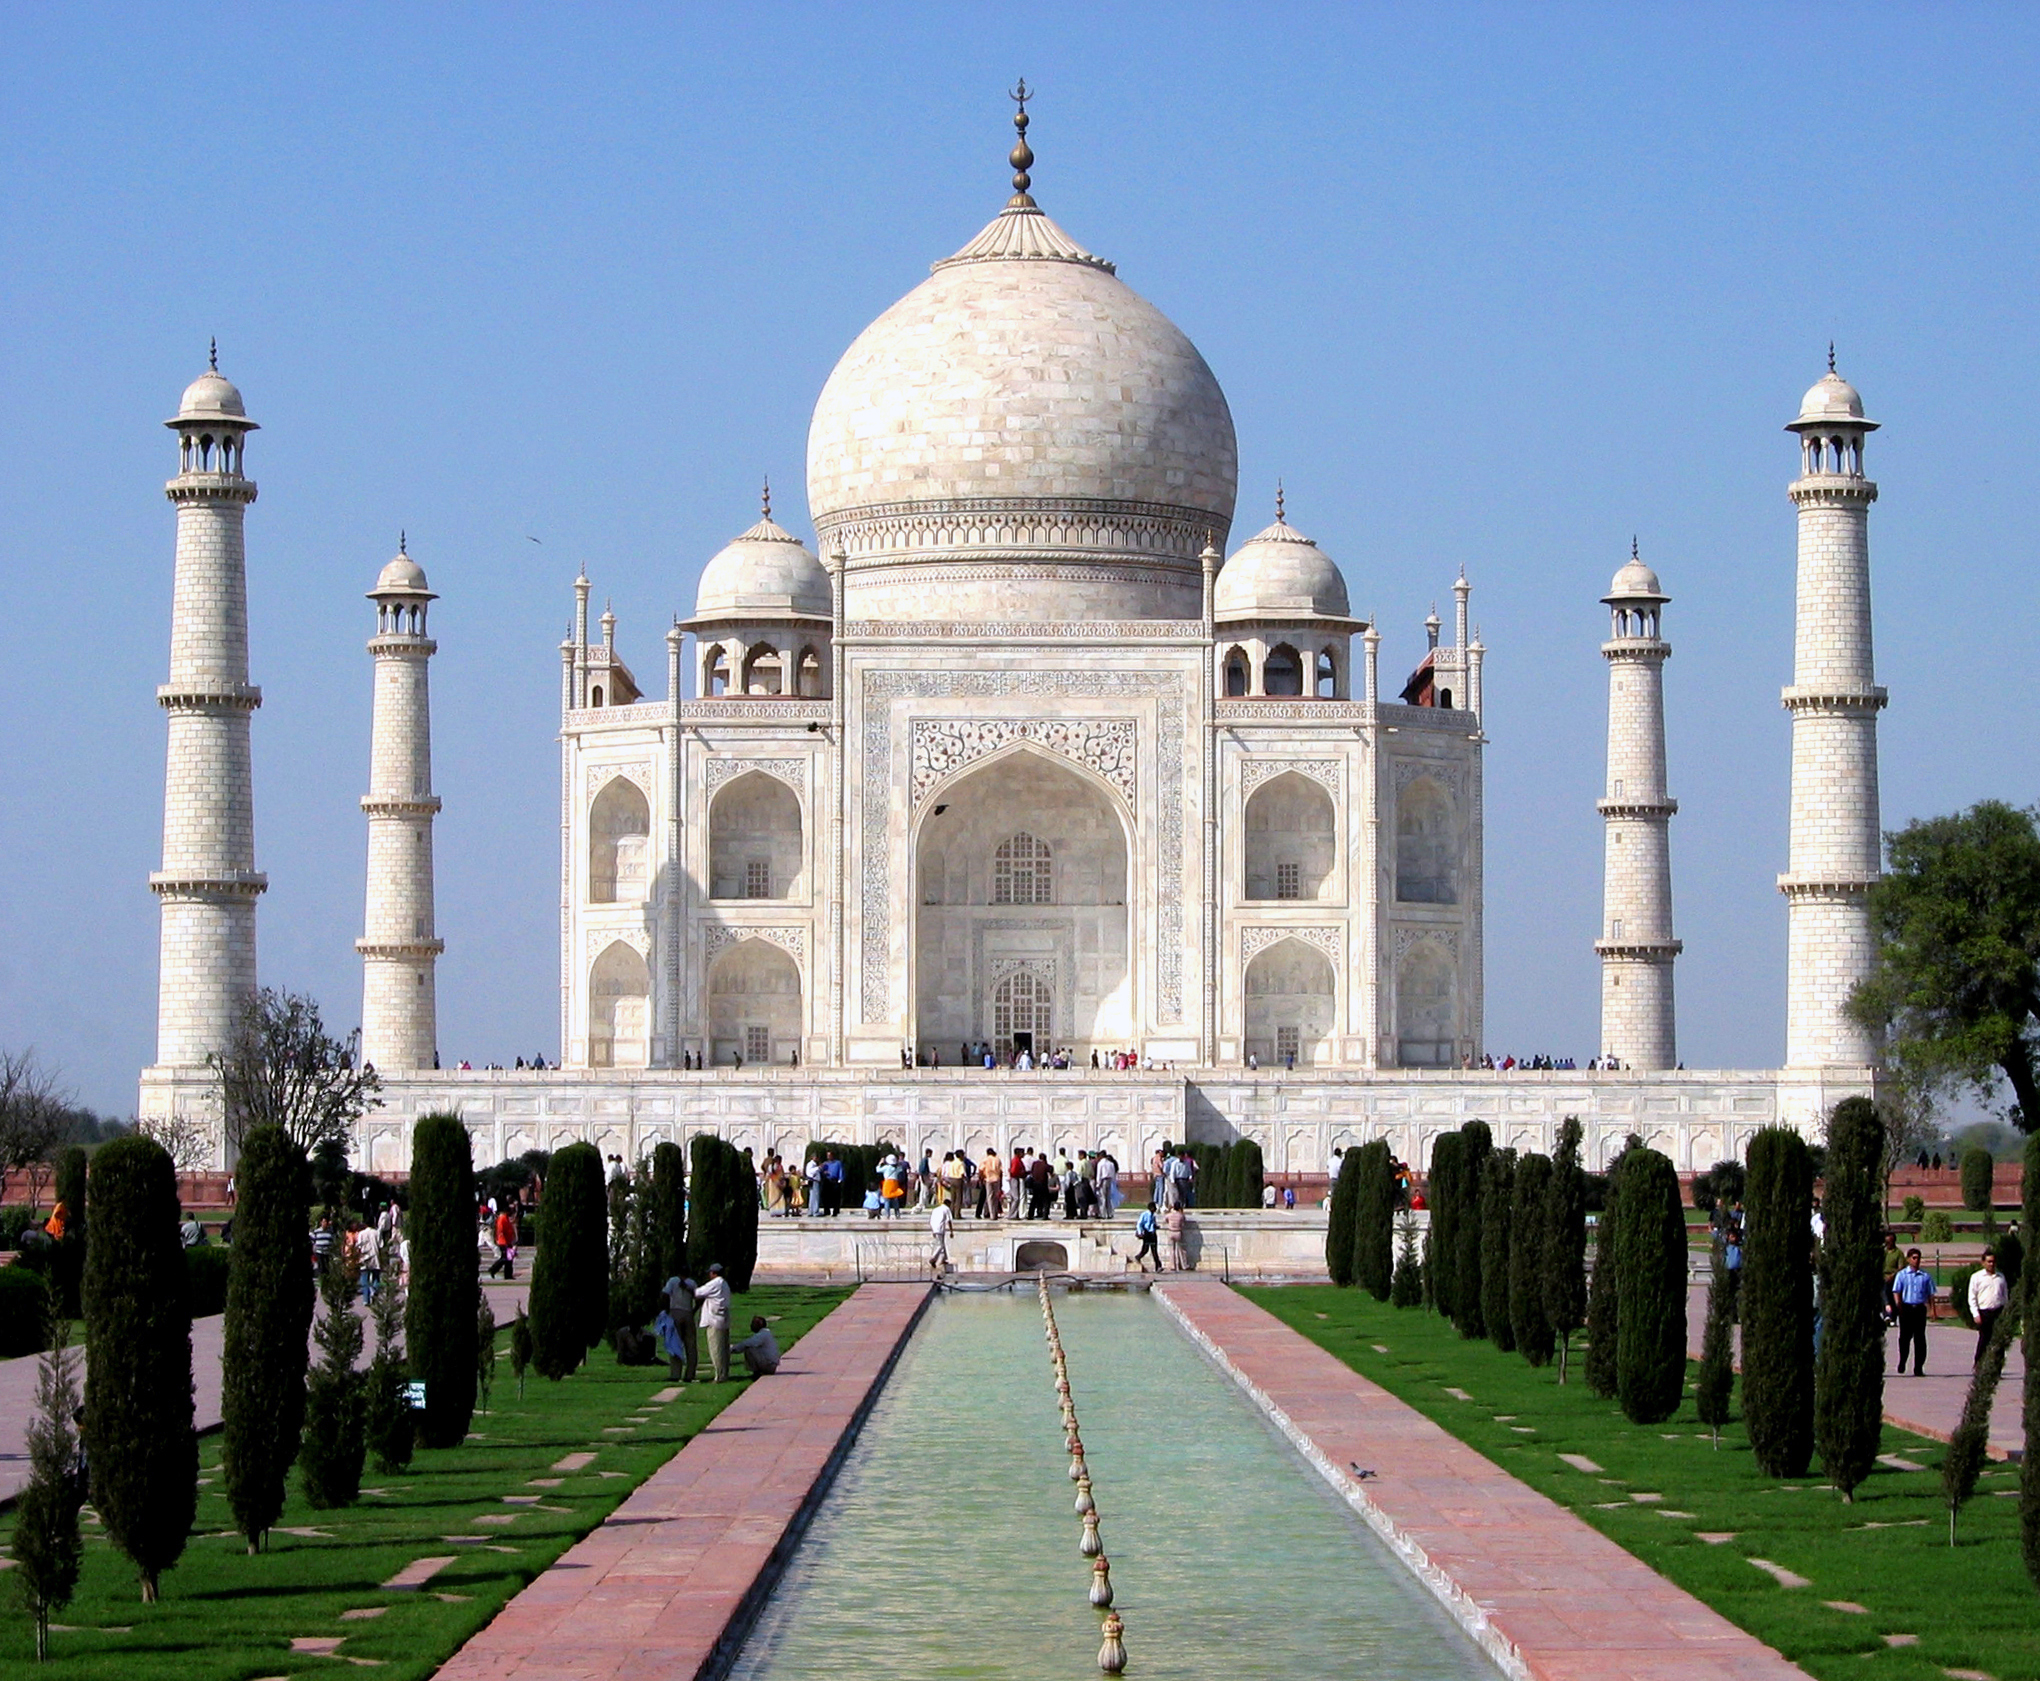
\includegraphics[width=20mm,scale=0.7]{images/taj_mahal.jpg}};}
	\onslide<5->{  \node [right=4.3cm of input_taj.south,anchor=south west] (edge)  { 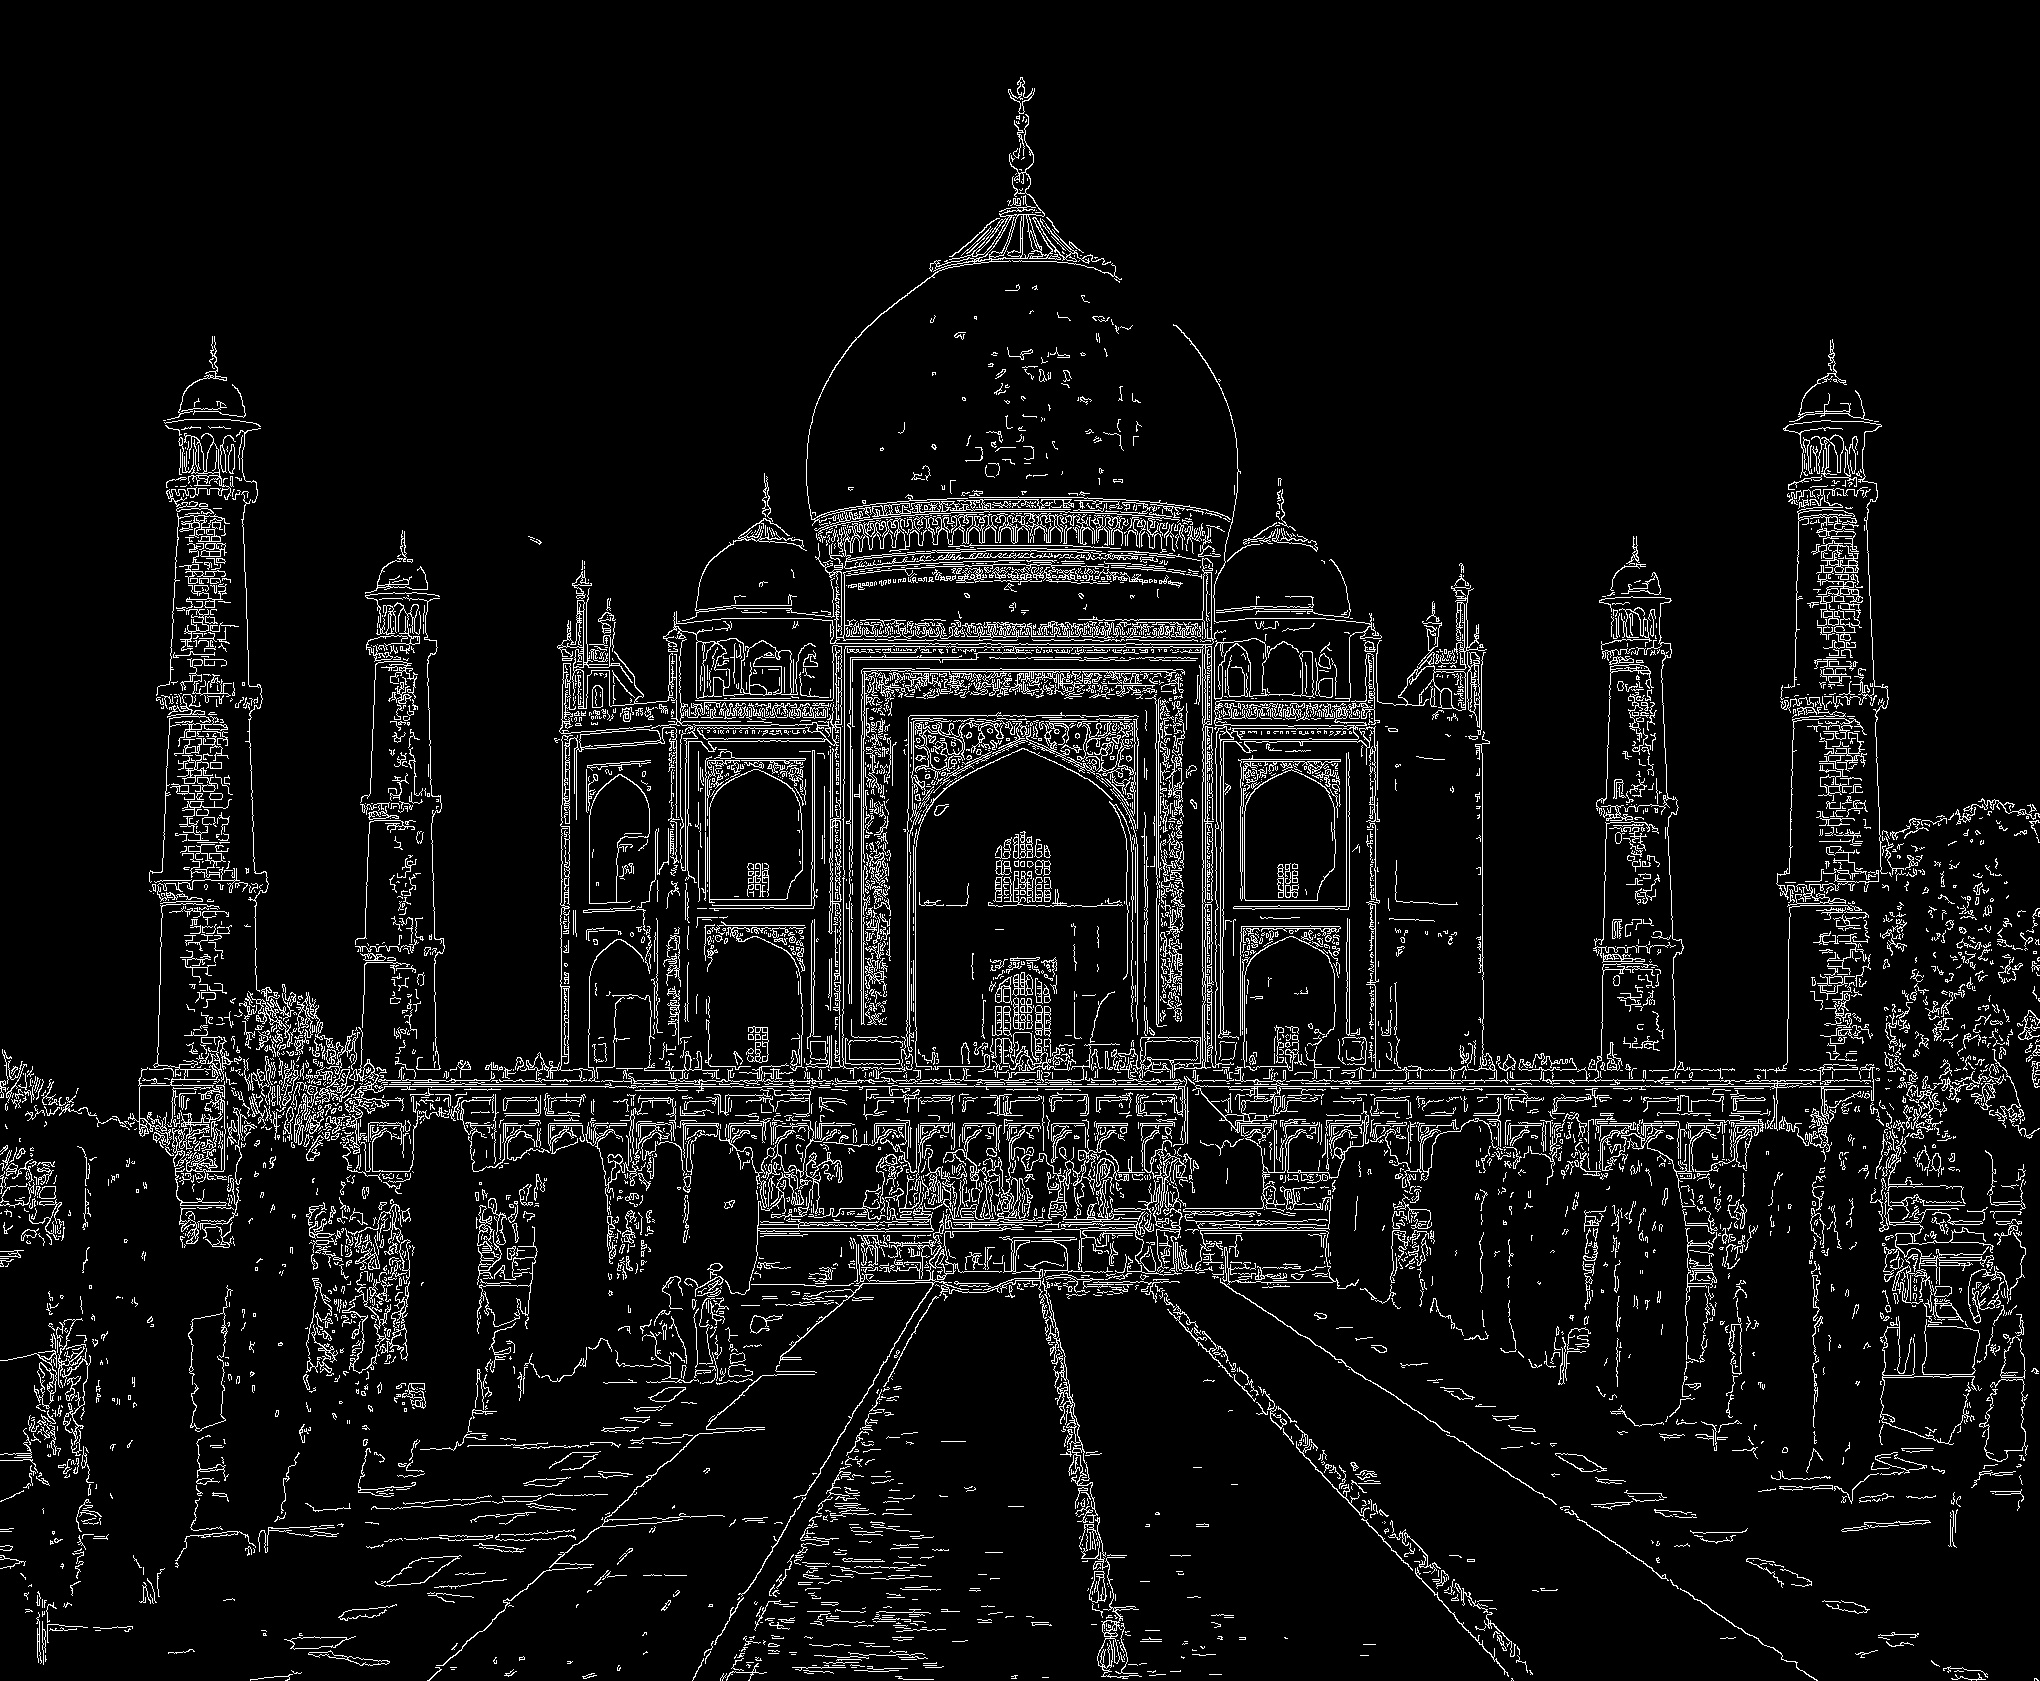
\includegraphics[width=20mm,scale=0.7]{images/taj_mahal_detectedges.jpg}};

		%\node[above of= raw,node distance=1.2cm ] (features)  {Features};
		\draw[->,thick] (input_taj) -- node [midway, above] {\footnotesize{$Edge\,Detector$}} (edge) ;}
	\onslide<6->{\node [right=5cm of edge.center,anchor= center](output_taj){car, bus, \textcolor{blue}{monument}, flower};
		\draw[->,thick] (edge) -- (output_taj) ;}

\end{tikzpicture}